\documentclass[11pt]{article}
\usepackage[utf8]{inputenc}
\usepackage[T1]{fontenc}
\usepackage[spanish,es-tabla]{babel} % idiomas (uno o varios)

\usepackage[left = 2.25cm, right = 2.25cm, top=1.5cm, bottom = 1.5cm]{geometry}
\usepackage{mathtools} % símbolos extensibles (contiene amsmath)
\usepackage{amssymb} % símbolos matemáticos
\usepackage{mathrsfs} % para usar \mathscr{}
\usepackage{physics} % notación de Dirac
\usepackage{tensor} % índices en cualquier lado

\usepackage{booktabs} % tablas
\usepackage[bookmarks = true, colorlinks=true, linkcolor = black, citecolor = black, menucolor = black, urlcolor = black]{hyperref} % para referencias cruzadas
\usepackage[table]{xcolor} % colores (incluye colortbl la cargarlo con table)
\usepackage{tcolorbox} % cajas de colores con titulo

\usepackage{float} % para figuras (las fija, [H], ...)
\usepackage{graphicx} % para figuras
\usepackage{caption} % pie de foto
\usepackage{subcaption} % pie de ''subfoto''


\selectlanguage{spanish}
\renewcommand{\theenumi}{\roman{enumi}}
\renewcommand{\thefigure}{\Roman{figure}} 
\newcommand\diagram[2]{\schema{\schemabox{#1}}{\schemabox{#2}}}

\begin{document}

\subsubsection*{Ejercicio 1}

\begin{figure}[H]
\centering
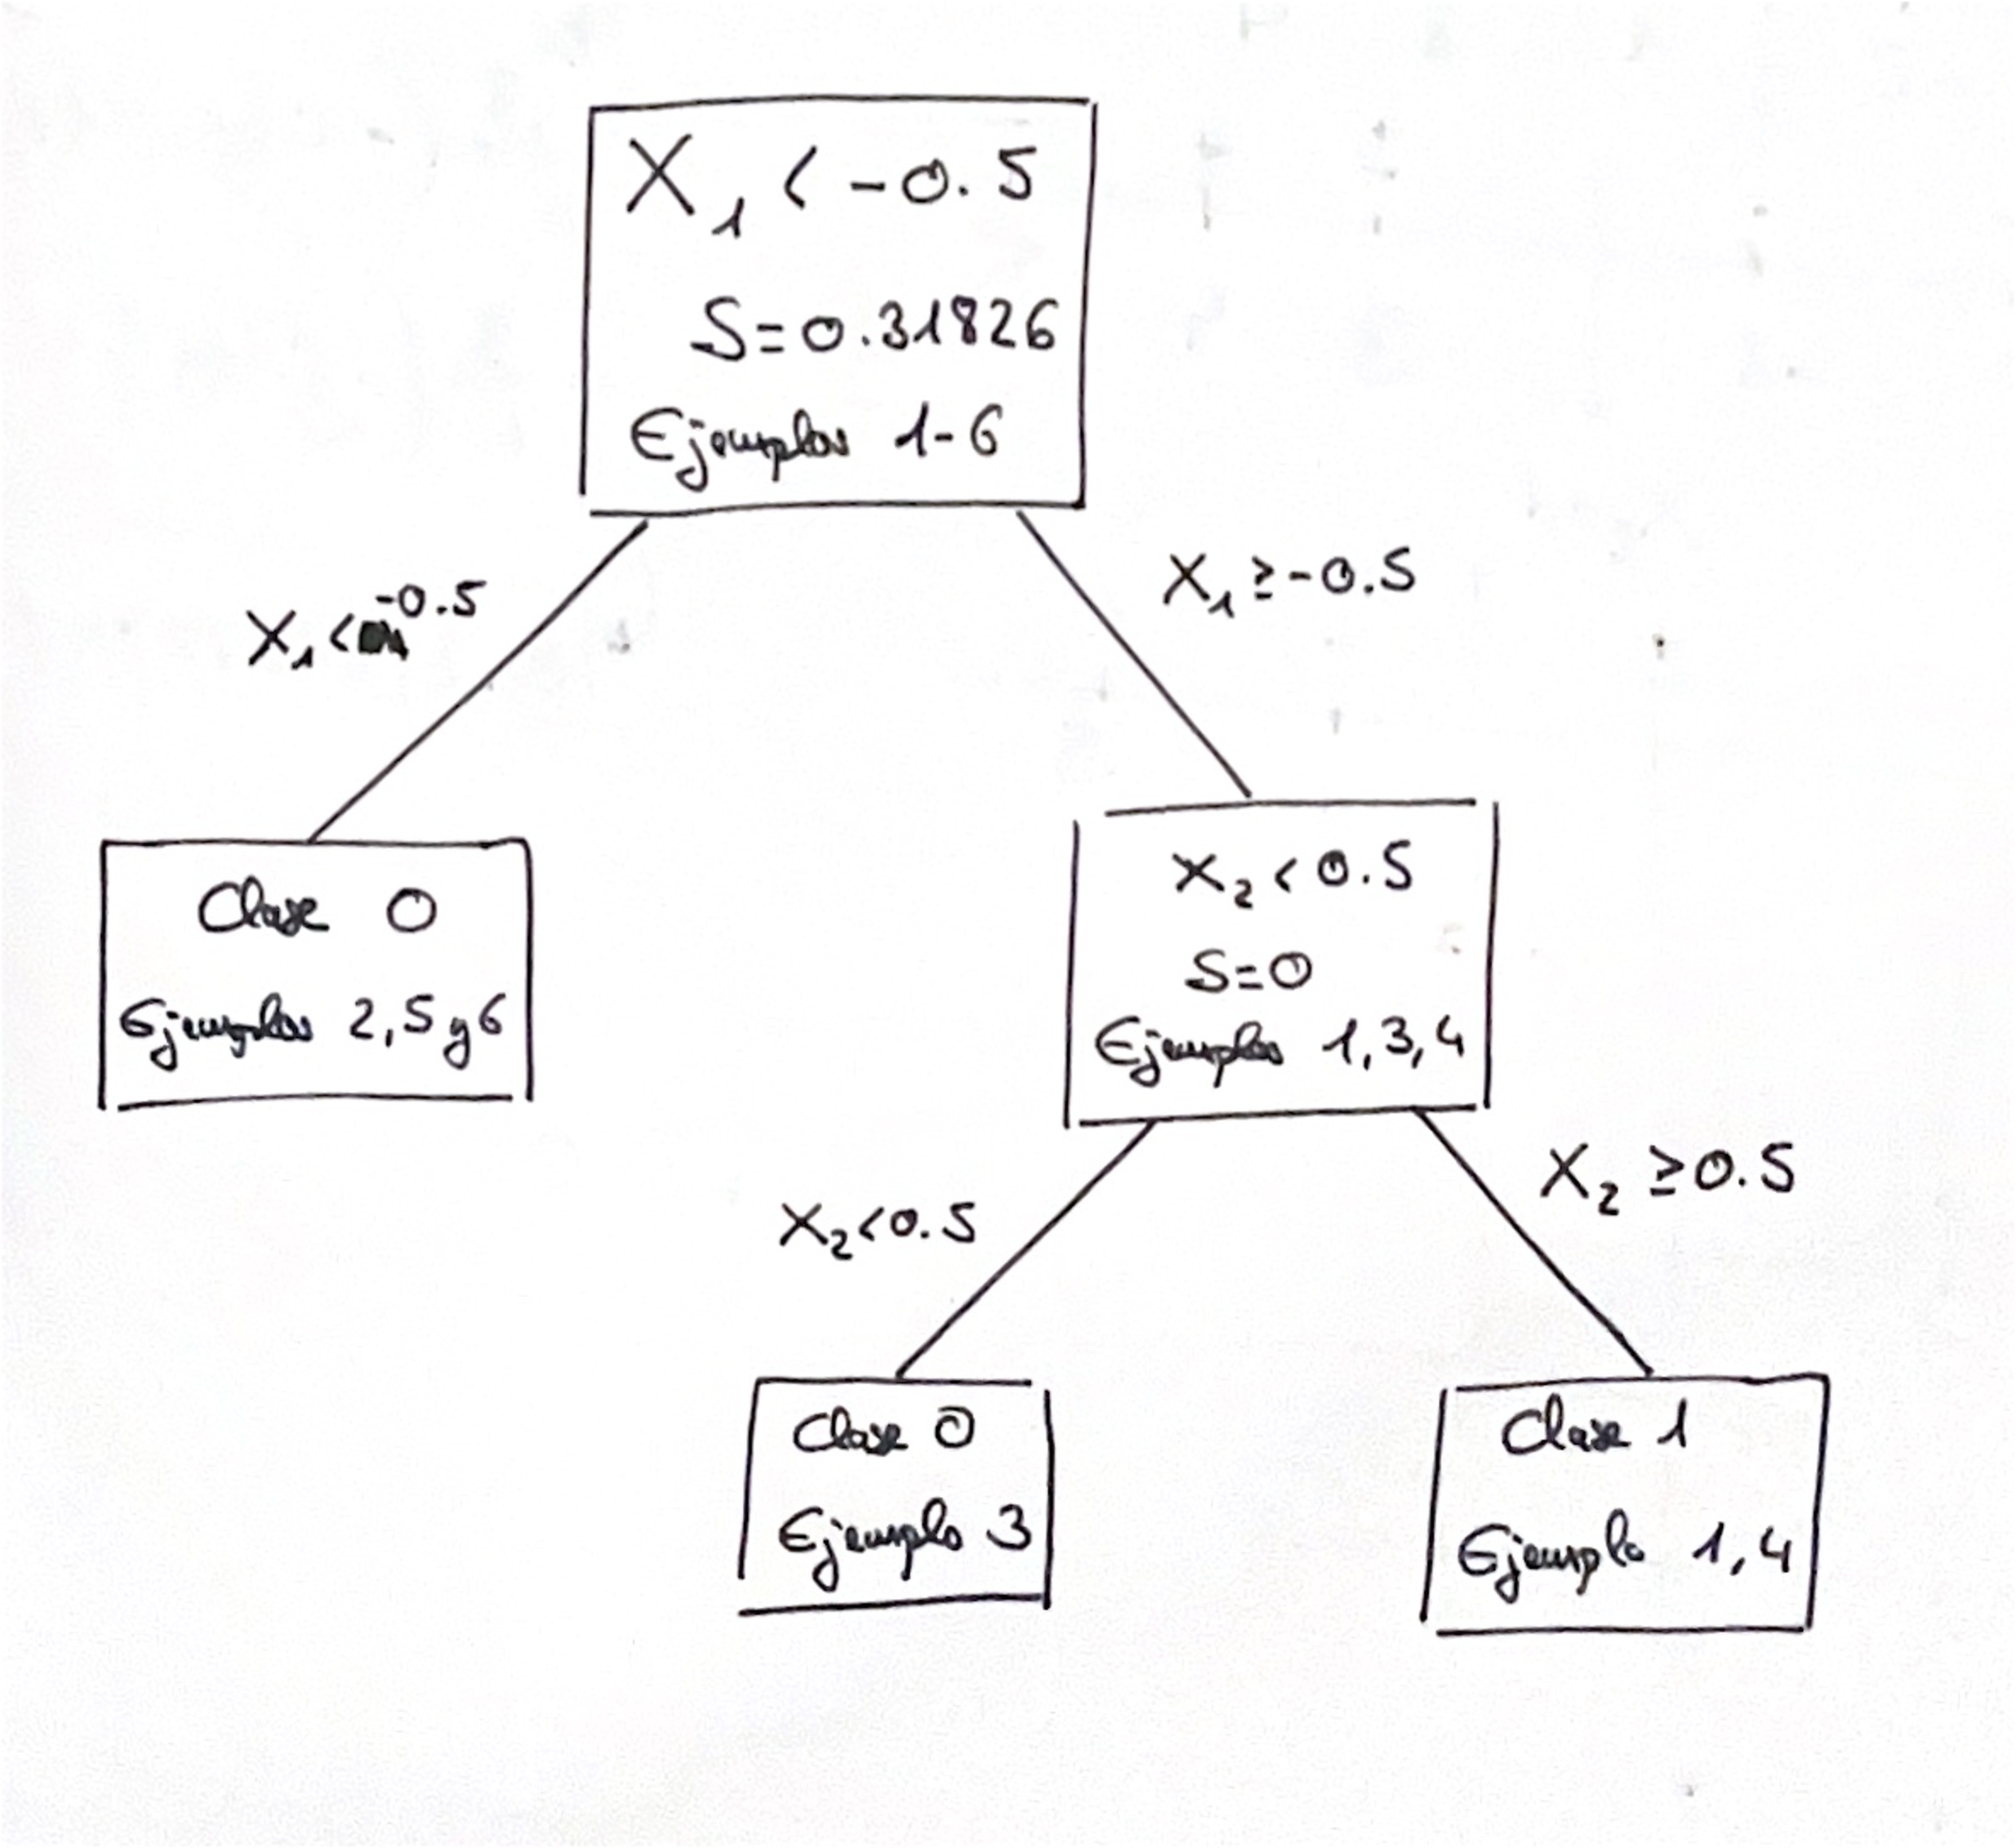
\includegraphics[width=0.5\textwidth]{fotos/arbol.pdf}
\end{figure}

\subsubsection*{Ejercicio 2}

\begin{itemize}
    \item \textbf{Menor error de validación cruzada, su desviación estándar y valor del hiperparámetro:} $\Delta = 0.217353$, $\sigma = 0.014349$, $\text{hy} = 110$.
    \item \textbf{Con regla de una desviación estándar:} $\Delta = 0.229118$, $\sigma = 0.019768$, $\text{hy} = 119$.
    \begin{figure}[H]
    \centering
    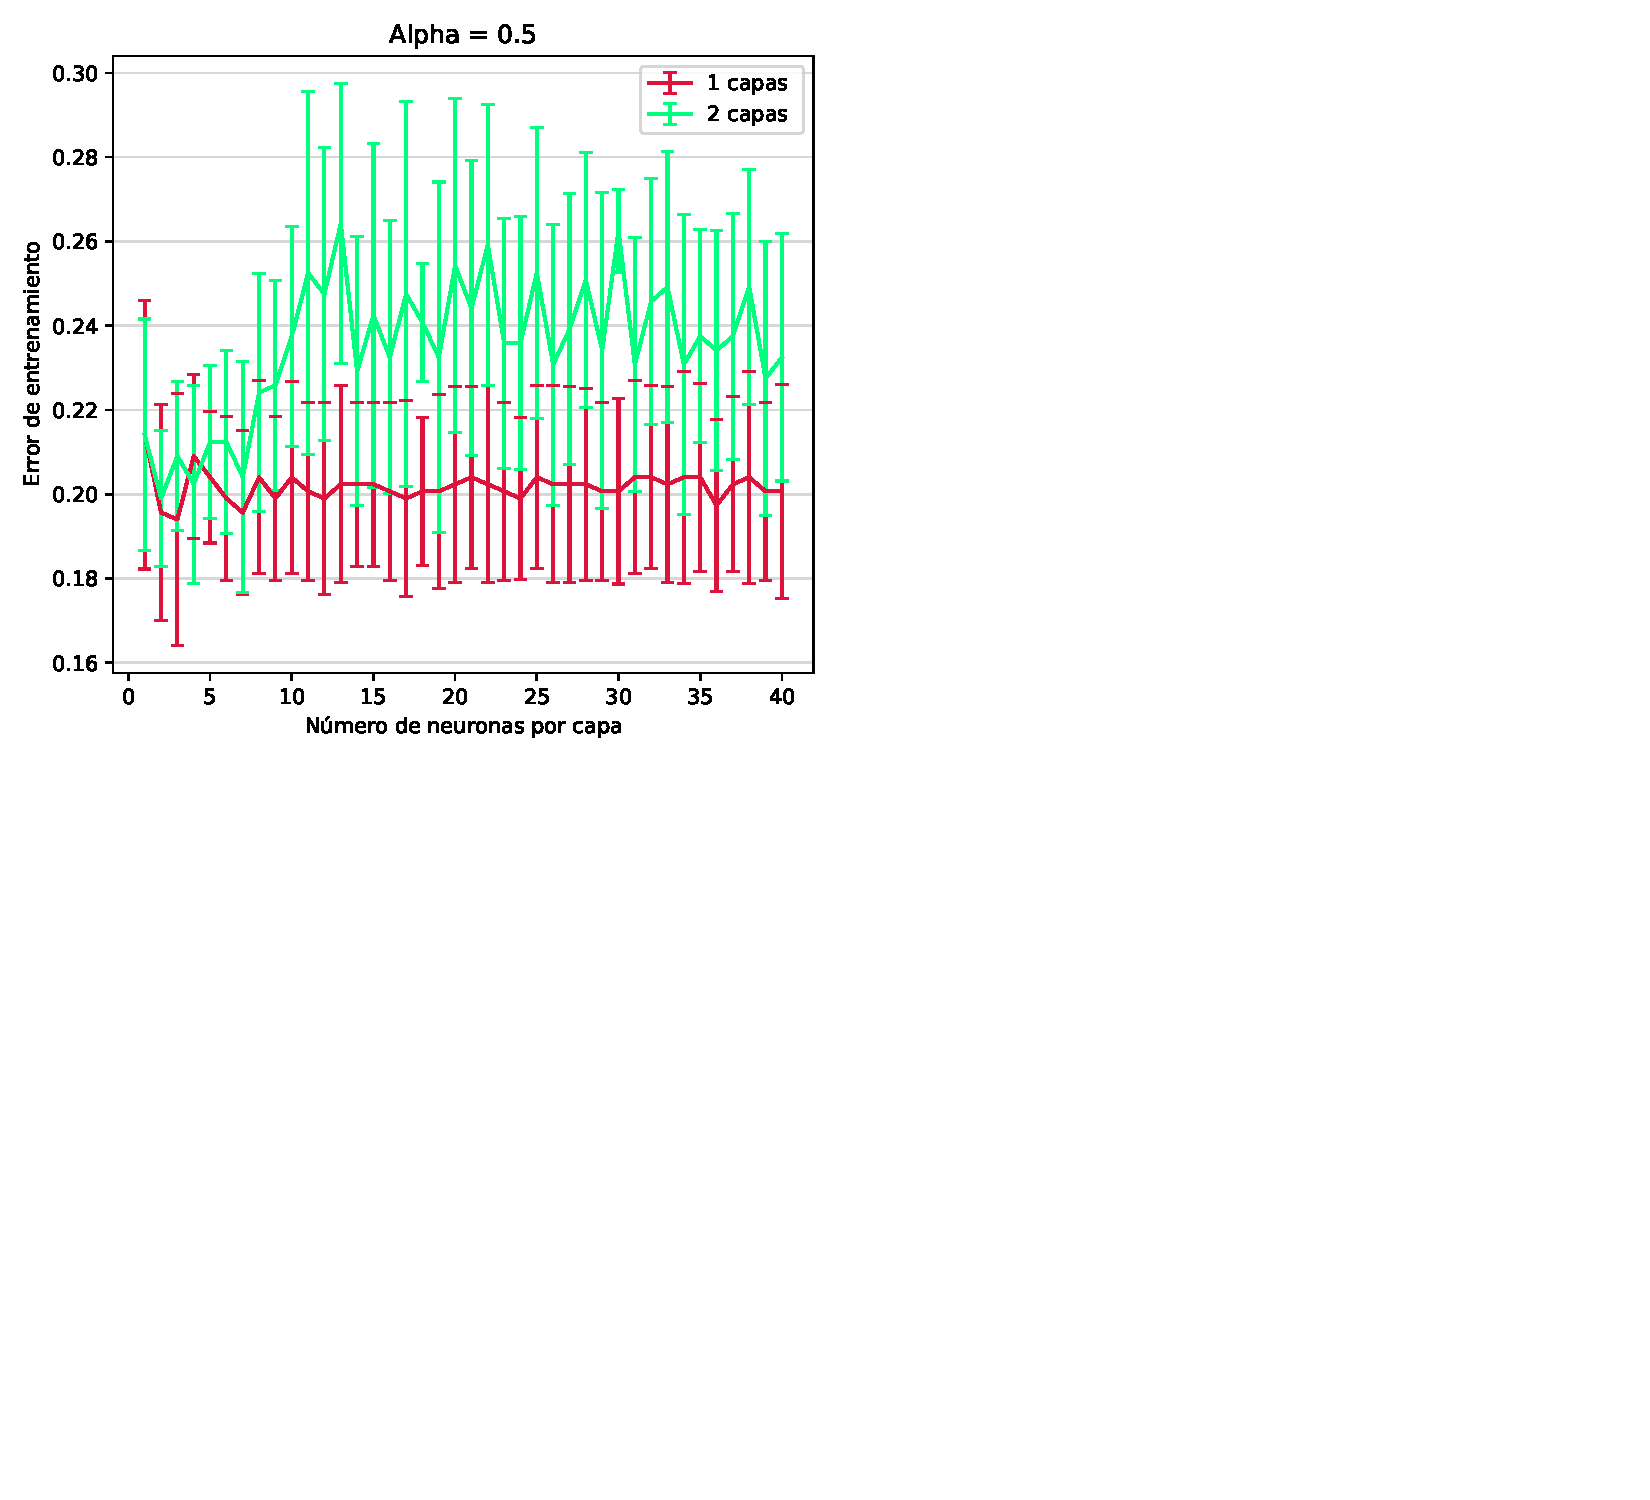
\includegraphics[width=0.9\textwidth]{fotos/ej2_1.pdf}
    \end{figure}
    \item \textbf{Error de test para el hiperparámetro de validación cruzada:} $\Delta = 0.253333$, $\text{hy} = 110$.
    \begin{figure}[H]
    \centering
    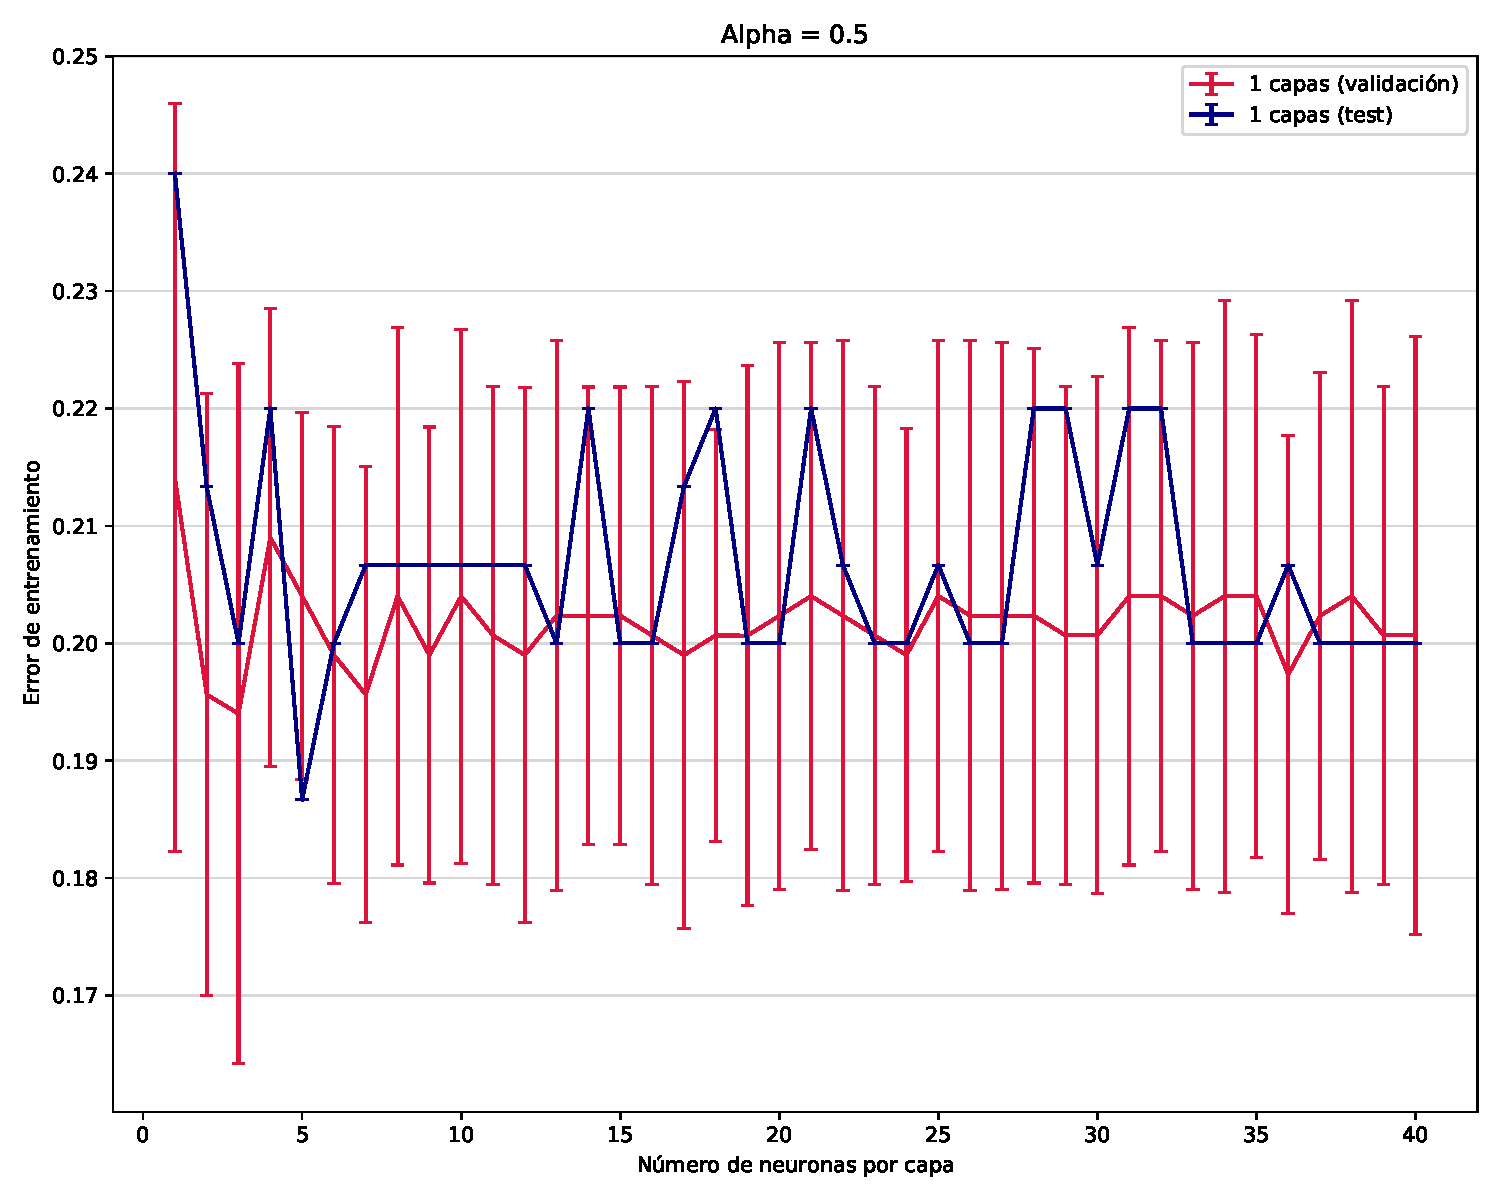
\includegraphics[width=0.9\textwidth]{fotos/ej2_2.pdf}
    \end{figure}
\end{itemize}


\subsubsection*{Ejercicio 3}

\begin{itemize}
    \item \textbf{Menor error de validación cruzada, su desviación estándar y valor del hiperparámetro:} $\text{MSE} = 3.400035$, $\sigma = 0.68836$, $\text{hy} = 15$.
    \item \textbf{Con regla de una desviación estándar:} $\text{MSE} = 4.024361$, $\sigma = 0.449845$, $\text{hy} = 35$.
    \begin{figure}[H]
    \centering
    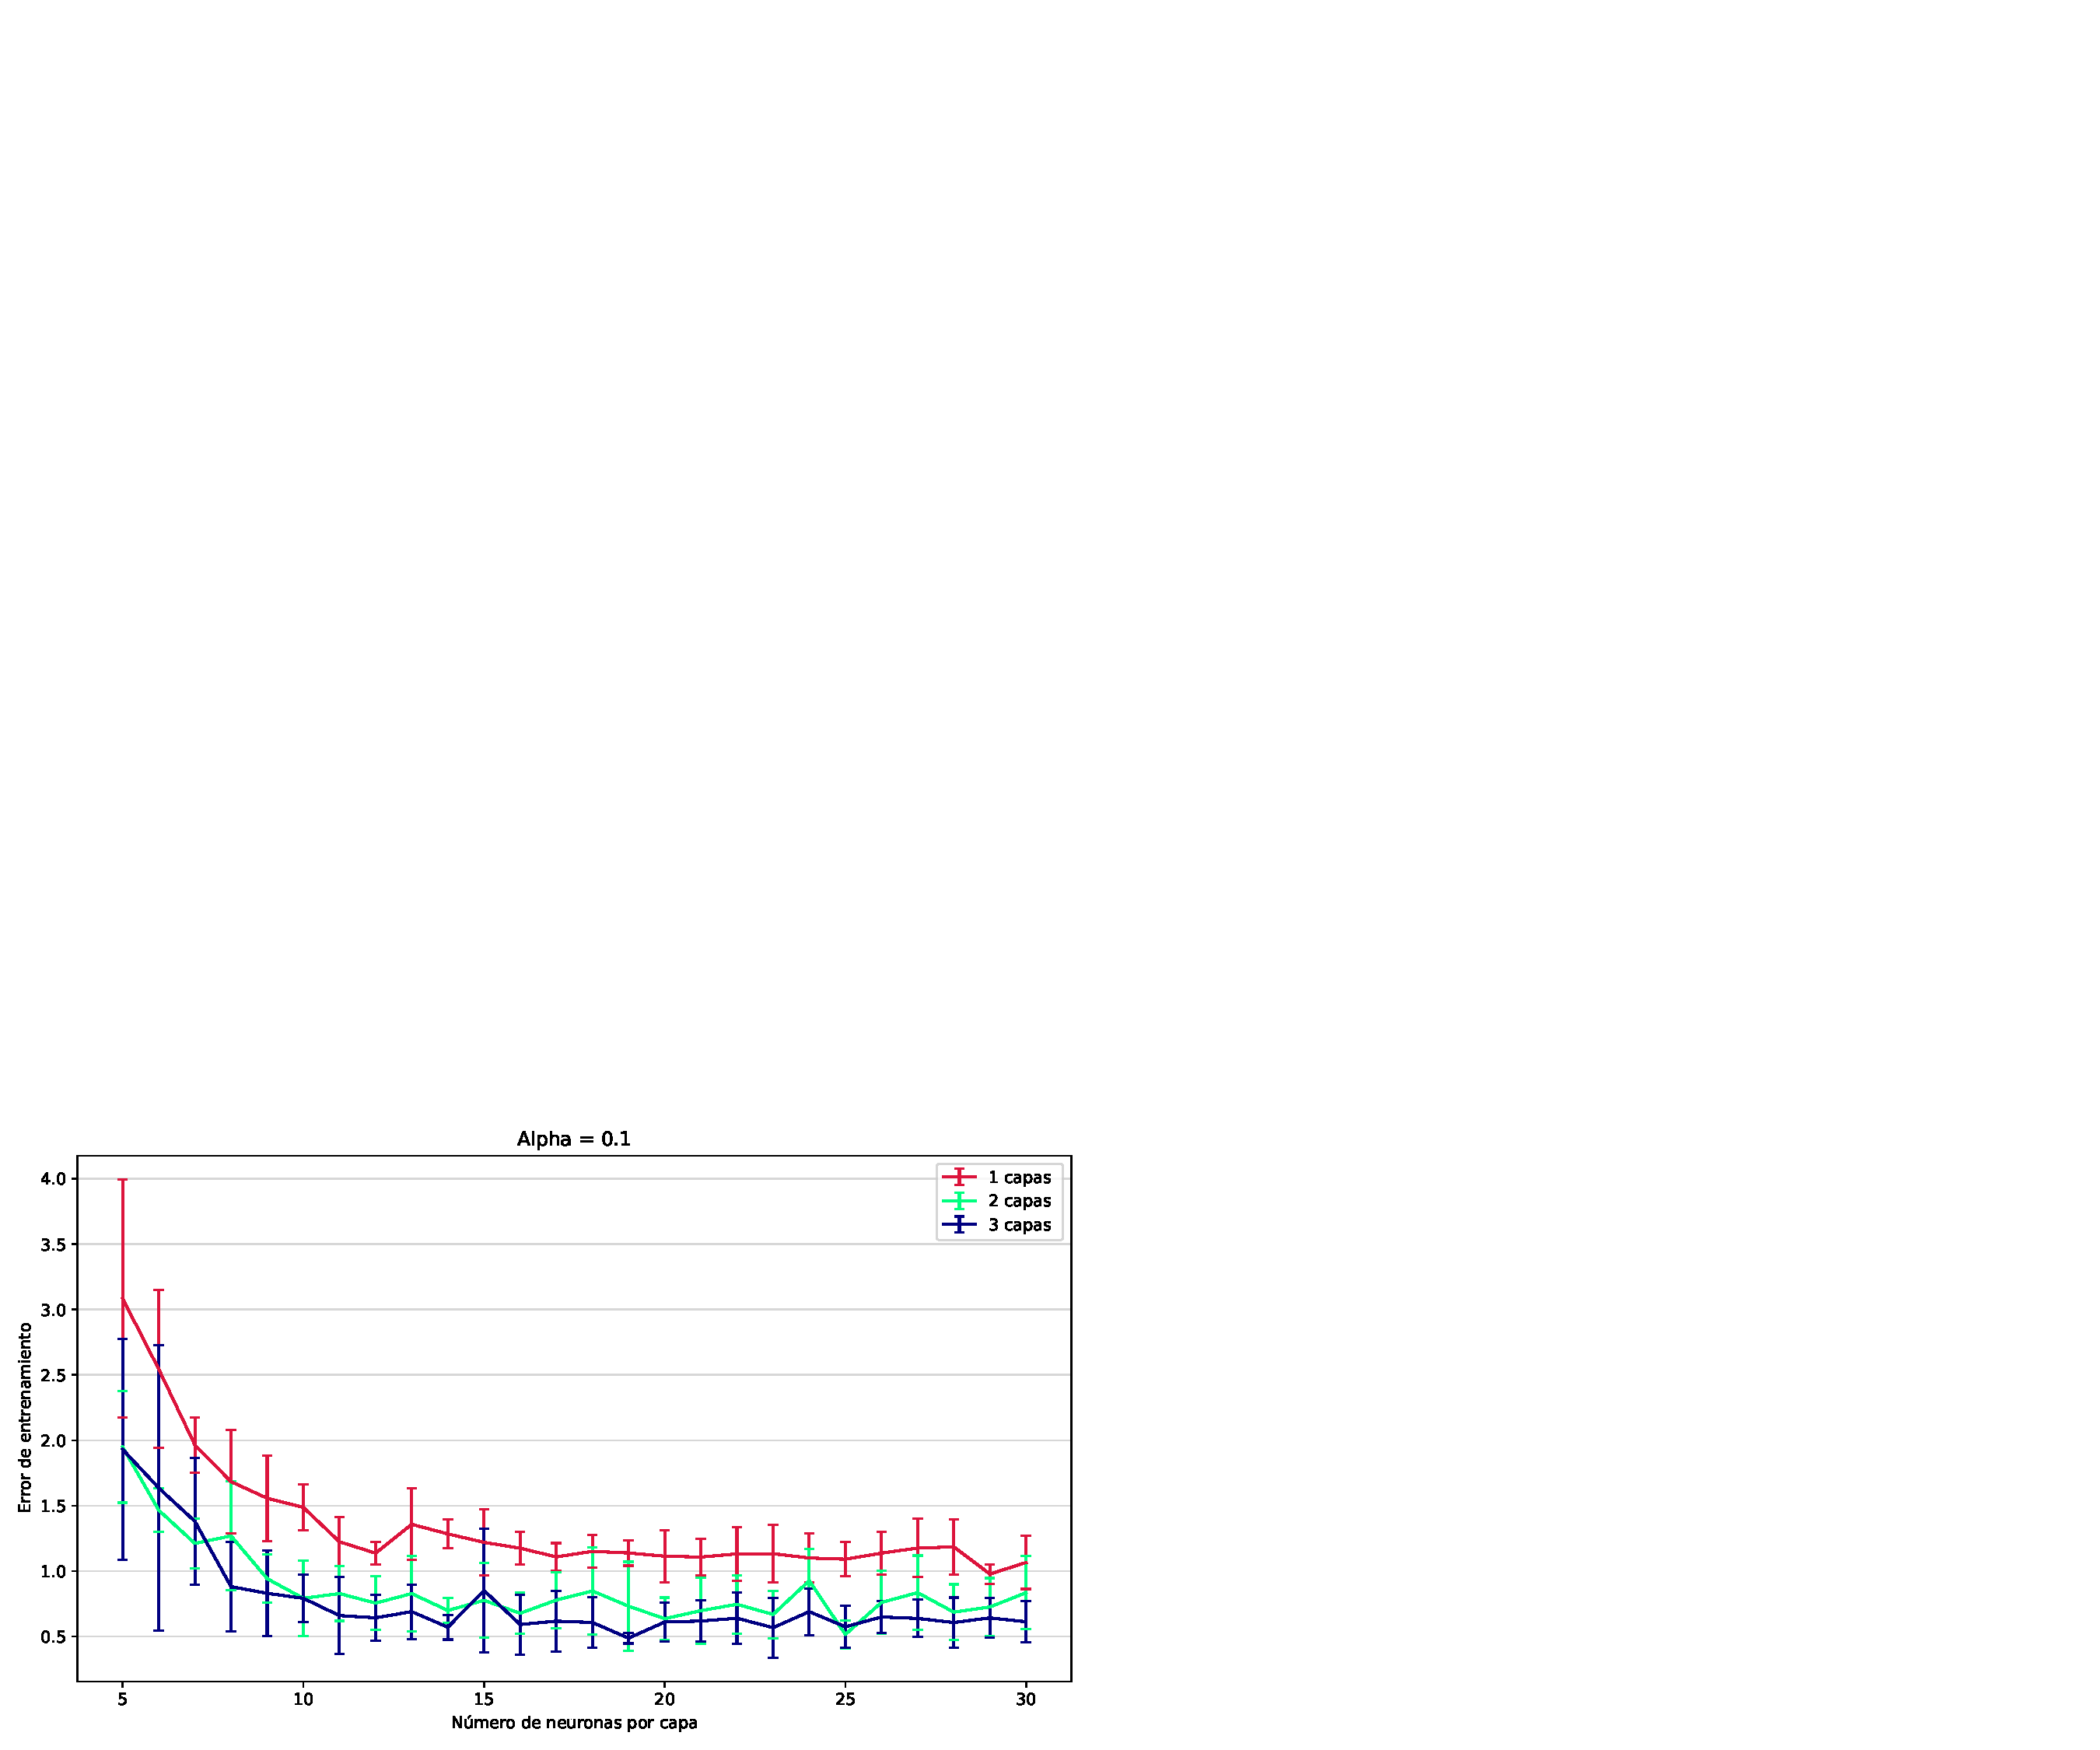
\includegraphics[width=0.75\textwidth]{fotos/ej3_1.pdf}
    \end{figure}
    \item \textbf{Error de test para el hiperparámetro de validación cruzada:} $\text{MSE} = 4.87007$, $\text{hy} = 15$.
    \begin{figure}[H]
    \centering
    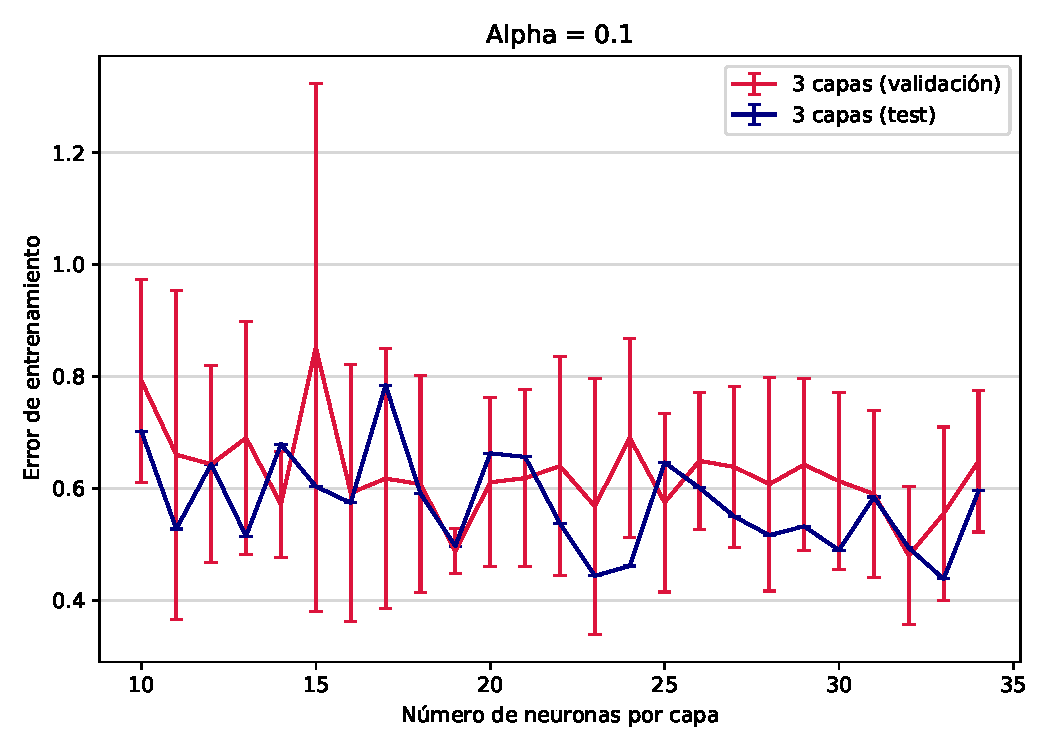
\includegraphics[width=0.75\textwidth]{fotos/ej3_2.pdf}
    \end{figure}
\end{itemize}


\end{document}
